\chapter{Background}
\label{chp:chapter_2}
In 1996, Intel, Ericsson, and Nokia came together with the goal of standardizing short-range radio technology for connectivity between different products across many industries. The resulting technology was codenamed Bluetooth, lending its name to King Harald ``Bluetooth'' Gormsson, who was known for uniting Denmark and Norway in 958 and, more importantly, for his dead blue tooth \cite{bluetooth_sig_name}. From this collaboration, the Bluetooth Special Interest Group (SIG) was formed, which released its first version of the standard in 1999. Today, Bluetooth SIG has over 36 thousand members \cite{bluetooth_sig_us}.

Bluetooth 4.0 first introduced Bluetooth Low-Energy (BLE) with a focus on low-power devices like wireless headphones and location beacons. BLE was not intended to replace the classic Bluetooth, now called Bluetooth Basic Rate/Enhanced Data Rate (BR/EDR), but to live alongside it and expand on the feature set available.

Since its inception, Bluetooth has become one of the most ubiquitous wireless communication technologies, reaching nearly 100\% market saturation in platform devices (phones, tablets, and PCs) \cite{bluetooth_market_update_2022}. In 2022, over 5.1 billion devices were shipped with Bluetooth radios, projected to grow to 7 billion by 2026. By that time, Bluetooth SIG expects 95\% of all Bluetooth devices to support the LE-variant, highlighting BLE's importance.

In this chapter, the background information will be covered to understand the architecture of the solutions proposed to fix the inefficiencies mentioned in Chapter \ref{chp:introduction}. This information includes a high-level overview of the BLE stack, an explanation of the Operating Systems (OS) used to implement the solutions, and some useful definitions. For a more comprehensive explanation of BLE and how to implement it, we refer to Getting Started with Bluetooth Low Energy \cite{townsend_cufi}.

\section{Wireless Connection}
\label{sec:ch2_wireless_connection}
Within the Bluetooth Low-Energy connection, there exists a clear hierarchy, where one device is dominant and is called the \textit{central}. The central is in control of the connection and is usually a phone or a laptop. The other side of the connection (one or more) is called the \textit{peripheral}. Typical peripheral devices include headphones, smart watches, IoT sensors, and push buttons. 

For this thesis, we define three phases for a BLE connection. These phases are:
\begin{itemize}
    \item \textit{Unconnected}: Before any connection is established between the central and the peripheral.
    \item \textit{Connection Setup}: Starts from the connection request and ends when the last non-application packet is sent. 
    \item \textit{Application}: Starts when connection setup is finished, and only application packets are sent. Application packets are packets that are necessary to fulfill the application. 
\end{itemize}
These terms are not officially defined by the BLE specification but are used throughout this thesis. 

\section{Connection Setup}
As previously defined in Section \ref{sec:ch2_wireless_connection}, the connection setup starts from the Connection Request and ends when the last non-application packet is sent. The packets that occur during Connection Setup can be divided into four groups which correspond to the subjects discussed in the previous sections.
\begin{itemize}
    \item Link Layer
    \item Service Discovery
    \item Configuration
    \item Application
\end{itemize} 
The order in which they occur is usually Service Discover, Configuration, and then Application, with Link Layer communication starting parallel to the Service Discovery from the start.

\section{Architecture of the Bluetooth Low-energy Stack}
\begin{figure}[]
    \centering
    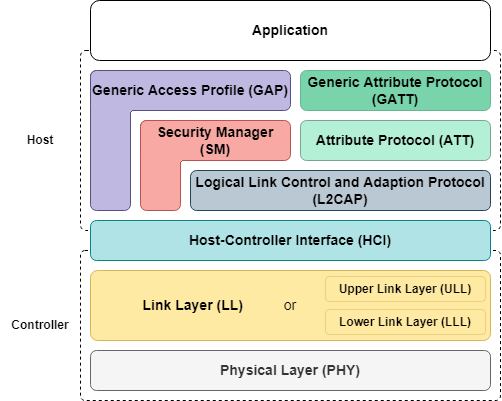
\includegraphics[width=0.8\textwidth,height=6cm,keepaspectratio=true]{images/ble_stack/ble_stack.drawio.png}
    \caption{
        The BLE Network Stack. The controller is comprised of the Physical Layer and the Link Layer. The Generic Access Profile, Security Manager, Generic Attribute Protocol, and Attribute Protocol messages get translated by the Logical Link Control and Adaption Protocol and together form the host. The Host-Controller Interface exists between the host and controller.
    }
    \label{fig:ble_stack}
\end{figure}

As seen in Figure \ref{fig:ble_stack}, the BLE stack is divided into many layers with increasing levels of abstraction. The bottom-most layers, the Physical Layer (PHY) and Link Layer (LL), form the controller, which is responsible for controlling the connection. The top-most layers, the Generic Access Profile (GAP), Security Manager (SM), Generic Attribute Protocol (GAP), and Attribute Protocol (GATT), provide higher level functionality and APIs which, together with the Logical Link Control and Adaption Protocol (L2CAP) form the host.

The separation of the host and controller is derived from how Bluetooth BR/EDR is implemented, where the host and controller can be implemented separately or even exist on different chips entirely. The host and controller are connected together using a Host-Controller Interface. This separation also allows a single radio to be used simultaneously with a BR/EDR and BLE controller and a generic host to support both versions of Bluetooth.

Nordic Semiconductors supplies the SoftDevice for its microcontrollers, which contains the host and controller in a single qualified, pre-compiled binary \cite{nordic_softdevices}. The Zephyr framework can interface with Nordic's SoftDevice Controller through HCI or, since version 3.0.0, supports its own custom Zephyr BLE Controller. Packetcraft implements the entire stack from application to PHY.

\subsection{Physical Layer}
\label{sec:phy_layer}
The PHY operates at the unlicensed 2.4GHz ISM (industrial, scientific, and medical) band and uses Gaussian frequency-shift keying (GFSK) modulation with adaptive frequency-hopping to reduce collisions. The 2.4GHz band is divided into 40 channels from 2.4000GHz to 2.4835GHz. The radio calculates the next hop using the formula:

\[\text{channel}_{\text{new}} = (\text{channel}_{\text{current}} + \text{hop}) \text{ modulo } 37\]
    
where the value \textit{hop} is exchanged when the connection is established.

BLE has a theoretical maximum throughput of 1Mbps for version 4.2 and 2Mbps for version 5.0. However, in practice, this lies much lower. In normal operation (uncoded), every bit is represented by one symbol. From version 5.0 onwards, BLE supports \textit{Coded PHY} where a single bit is represented by 2 to 8 symbols for improved range but reduced throughput.

\subsection{Link Layer} 
The link layer (LL) directly controls the PHY and manages the link state. The link layer is the only hard real-time layer of the BLE stack and is partly hardware dependent. For this reason, it is usually implemented and kept separate from the rest of the stack. However, Zephyr goes even further and splits the link layer into an upper and a lower link layer (ULL and LLL, respectively), where the ULL is hardware agnostic and generic, and the LLL is hardware specific.

\subsubsection{States and Roles}
\begin{figure}[]
    \centering
    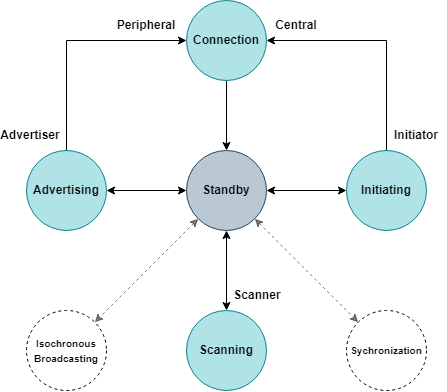
\includegraphics[width=0.8\textwidth,height=6cm,keepaspectratio=true]{images/ll_states/ll_states.drawio.png}
    \caption{
        Link Layer state machine diagram. In the standby state, no packets are received or transmitted. Advertisers send advertising packets without a connection, scanners receive advertising packets without the intention of connecting, and initiators initiate a connection with advertisers, which then become the centrals and peripherals, respectively.
    }
    \label{fig:ll_states}
\end{figure}
The link layer can be described as a system of one or more state machines. The states that each LL state machine can occupy are shown in Figure \ref{fig:ll_states}. The link layer should have at least one LL state machine that supports \textit{Advertising} or \textit{Scanning}. 

The link layer in \textit{standby} does not receive or transmit any packets. When the link layer moves from \textit{standby} to \textit{advertising}, the link layer takes on the role of \textit{advertiser}. As an advertiser, the link layer transmits advertising channel PDUs and possibly responds to requests from other devices for more data. The different types of advertising packets and their content will be discussed later.

A link layer in the \textit{scanning} state takes on the role of a \textit{scanner}. In this role, it can listen for advertising packets and consume their content, but it can not form a connection with the \textit{advertiser}.

If a device intends to form a connection with an advertiser, it should enter the \textit{intitiating} state, taking on the role of \textit{initiator}. When an advertisement packet is received, the \textit{initiator} can respond with a \texttt{CONNECT\_IND} packet to form a connection. After a connection is formed, the \textit{initiator} becomes the \textit{central} and the \textit{advertiser} becomes the \textit{peripheral}. The \textit{central} defines the timing of transmission events.

The \textit{synchronization} state is used to listen to periodic advertising trains from a specific device within its \textit{Broadcast Isochronous Group} (BIG). The \textit{isochronous broadcasting} state is used to broadcast data to a group of devices in a BIG. These states are used when a single device continuously streams data to multiple receivers, such as wireless earphones. Figure \ref{fig:ll_states} shows these states with dotted borders since they do not apply to this thesis.

\subsubsection{Advertising and Scanning}
\begin{table}
    \begin{center}
    \begin{tabular}{|l|l|l|l|}
        \hline
        \textbf{Advertising Type} & \textbf{Connectable} & \textbf{Scannable} & \textbf{Directed} \\
        \hline
        \texttt{ADV\_IND} & Yes & Yes & No \\
        \hline
        \texttt{ADV\_DIRECT\_IND} & Yes & No & Yes \\
        \hline
        \texttt{ADV\_NONCONN\_IND} & No & No & No \\
        \hline
        \texttt{ADV\_SCAN\_IND} & No & Yes & No \\
        \hline
    \end{tabular}
    \end{center}
    \caption{Primary advertising PDU types.}
    \label{tbl:adv_types}
\end{table}

As an advertiser, the device sends out advertising channel packets at a set interval between 20ms and 10.240ms. The advertiser does this for device discovery, to broadcast data or both. There are four primary types of advertisement packet types. These types are shown in Table \ref{tbl:adv_types}.

These advertisement types can have three traits: \textit{connectable}, \textit{scannable} and \textit{directed}. A connectable advertisement type allows initiators to establish a connection using the \texttt{CONNECT\_IND} PDU. Packet types without the connectable trait are only used to broadcast data.

\begin{figure}[]
    \centering
    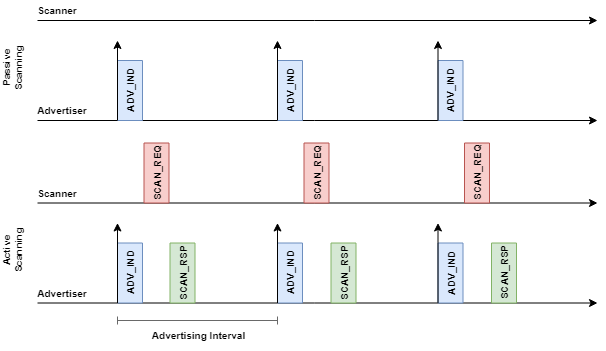
\includegraphics[width=0.6\textwidth,height=6cm,keepaspectratio=true]{images/scanning_modes/scanning_modes.drawio.png}
    \caption{When a scanner receives a scannable advertisement PDU while passively scanning, no further action is performed. However, when actively scanning, the scanner will perform a \textit{Scan Request}, forcing the advertiser to send more data in the form of a \textit{Scan Response}.}
    \label{fig:scan_modes}
\end{figure}
A scannable advertisement type allows a scanner or an initiator to request more data from the advertiser using a \textit{scan request} or \texttt{SCAN\_REQ} PDU. This forces the advertiser to respond with a \textit{scan response} or \texttt{SCAN\_RSP} PDU, which doubles the amount of data that can be broadcast. In this process, the scanner or initiator is said to perform \textit{active scanning}. On the contrary, \textit{passive scanning} is where the scanner or initiator only listens to advertisement packets and never issues a scan request. The difference between active and passive scanning is show in Figure \ref{fig:scan_modes}

A scanning device can listen for these packets and do nothing, which is called \textit{passive scanning}, or can request more data with a \textit{Scan Request}, which is called \textit{active scanning}. 

\newcommand{\bitlabel}[2]{%
    \bitbox[]{#1}{%
        \raisebox{0pt}[4ex][0pt]{%
            \turnbox{45}{\fontsize{7}{7}\selectfont#2}%
        }%
    }%
}
\newcommand{\textlabel}[2]{%
    \bitbox[]{#1}{\fontsize{7}{7}\selectfont#2}%
}

\begin{figure}
    \begin{center}
        \begin{bytefield}[bitwidth=2em]{16}
            \bitbox[]{1}{}\bitbox[]{5}{\textbf{Avertisement PDU}} \\ [1ex]
            \bitbox[]{1}{\textbf{a}}\bitbox{4}{Header (2 bytes)} \bitbox{12}{Payload (1-255 bytes)} \\
            \bitbox[]{1}{}\textlabel{4}{6 bytes} \textlabel{12}{0-31 bytes} \\ [3ex]

            \bitbox[]{1}{}
            \bitbox[]{3}{\textbf{Header}}
            \bitbox[]{1}{}
            \bitlabel{1}{RFU}
            \bitlabel{1}{ChSel}
            \bitlabel{1}{TxAdd}
            \bitlabel{1}{RxAdd} \\ [-1.75ex]
            \bitbox[]{1}{}\bitheader[endianness=little]{0-15} \\
            \bitbox[]{1}{\textbf{b}}\bitbox{4}{PDU Type}
            \bitbox{1}{}
            \bitbox{1}{}
            \bitbox{1}{}
            \bitbox{1}{}
            \bitbox{8}{Length}
        \end{bytefield}
    \end{center}
    \caption{a) Layout of the advertising PDU. b) layout of the advertisement PDU header. PDU Type as defined in Table \ref{tbl:adv_types}. The Length field contains the length of the Payload field in bytes.}
    \label{fig:adv_pdu}
\end{figure}

Figure \ref{fig:adv_pdu} shows the content of a generic advertising channel PDU. The first two bytes of the PDU contain the header, followed by 1 to 255 bytes of payload data. The four least significant bits of the header define the type of the advertising channel PDU and refers to the types defined in Table \ref{tbl:adv_types}. The \texttt{length} field contains the length of the Payload field in bytes.

\begin{figure}
    \begin{center}
        \begin{bytefield}[bitwidth=2em]{16}
          \bitbox[]{1}{} \bitbox[]{16}{\textbf{Payload} for \texttt{ADV\_IND}, \texttt{ADV\_DIRECT\_IND}, \texttt{ADV\_NONCONN\_IND}, and  \texttt{ADV\_SCAN\_IND} PDUs} \\
          \bitbox[]{1}{\textbf{a}}\bitbox{4}{AdvA} \bitbox{12}{AdvData} \\
          \bitbox[]{1}{} \textlabel{4}{6 bytes} \textlabel{12}{0-31 bytes} \\ [-1ex]

          \bitbox[]{1}{} \bitbox[]{3}{\textbf{AdvData}} \\
          \bitbox[]{1}{\textbf{b}} \bitbox{4}{AD Structure 1} \bitbox{4}{\ldots} \bitbox{4}{AD Structure $N$} \\ [1.4ex]

          \bitbox[]{1}{}\bitbox[]{4}{\textbf{AD Structure}} \\
          \bitbox[]{1}{\textbf{c}}\bitbox{2}{Length} \bitbox{2}{AD Type} \bitbox{5}{AD Data} \\
          \bitbox[]{1}{}\textlabel{2}{1 byte} \textlabel{2}{1 byte} \textlabel{5}{Length - 1 bytes}
        \end{bytefield}
    \end{center}
    \caption{a) Advertising channel PDU payload for advertising types of Table \ref{tbl:adv_types}. b) AdvData can contain as many AD Structures (contained pieces of advertisement data) as fits in 31 bytes. c) The AD Structure starts with the length of the AD Type (type of advertisement data as defined as defined in the Core Specification Supplement \cite{bluetooth_supplement}) and AD Data fields combined, followed by the AD Type, and finally, the AD Data as defined in the specification for that AD Type.}
    \label{fig:adv_payload}
\end{figure}

\begin{figure}
    \begin{center}
        \begin{bytefield}[bitwidth=1.5em]{12}
          \bitbox[]{8}{\textbf{Payload} for \texttt{SCAN\_REQ} PDU} \\
          \bitbox{6}{AdvA} \bitbox{6}{AdvData} \\
          \textlabel{6}{6 bytes} \textlabel{6}{6 bytes}
        \end{bytefield}
    \end{center}
    \caption{The Payload field of a \textit{Scan Request} or \texttt{SCAN\_REQ} PDU consists of ScanA and AdvA fields. The ScanA field contains the address of the scanner, and the AdvA field contains the address of the scanner.}
    \label{fig:scan_req_payload}
\end{figure}

The payload for the four advertising channel PDU types defined in Table \ref{tbl:adv_types} is shown in Figure \ref{fig:adv_payload}a. As seen in Figure \ref{fig:adv_payload}b, \textit{AdvData} can contain any number of \textit{AD Structures}. The AD Structure's \texttt{AD Type} field is an 8-bit identifier that refers to one of the many predefined advertisement datatypes. This is followed by the length of the data for this type and then the actual data. The payload of the scan request is shown in Figure \ref{fig:scan_req_payload}. The payload contains a \textit{ScanA} and \textit{AdvA} field, which contain the address of the scanner and advertiser, respectively. The payload of the \textit{Scan Response} or \texttt{SCAN\_RSP} PDU is the same as the advertising channel PDUs in Figure \ref{fig:adv_payload}.

Some examples of AD Types include \textit{Local Name}, \textit{TX Power Level}, and \textit{Appearance}. The \textit{Local Name} type allows the device to share its locally assigned device name. For example, one might name its headphones ``John's oPods'', which scanners can display to the user to identify the device. The \textit{TX Power Level} type can be used to calculate a rough distance estimation between the advertiser and the scanner, and the \textit{appearance} type can tell scanners the general appearance of the advertiser (smartwatch, for example).

\subsubsection{Connection Setup and Parameters}
The connection setup is initiated by the central by responding to an advertising channel PDU (for example, \texttt{ADV\_IND}) from an advertiser with a \textit{Connection Request} or \texttt{CONNECT\_IND} PDU. From this moment, a connection between the devices is made, and the setup can begin. If the central receives no empty PDU back as an acknowledgment of the connection request, then the central will retry for a specific (user-defined) number of attempts.

\newcommand{\bitboxsmalltext}[2]{%
    \bitbox{#1}{\fontsize{5}{5}\selectfont#2}%
}

\begin{figure}
    \begin{center}
        \begin{bytefield}[bitwidth=3em]{11}
          \bitbox[]{1}{} \bitbox[]{4}{\textbf{Payload} for \texttt{CONNECT\_IND} PDU} \\
          \bitbox[]{1}{\textbf{a}} \bitbox{2}{InitA} \bitbox{2}{AdvA} \bitbox{2}{LLData} \\
          \bitbox[]{1}{} \textlabel{2}{6 bytes} \textlabel{2}{6 bytes} \textlabel{2}{6 bytes} \\ [-1ex]

          \bitbox[]{1}{} \bitbox[]{3}{\textbf{LLData}} \\
          \bitbox[]{1}{\textbf{b}} 
          \bitbox{1}{AA}
          \bitboxsmalltext{1}{CRCInit}
          \bitboxsmalltext{1}{WinSize}
          \bitboxsmalltext{1}{WinOffset}
          \bitboxsmalltext{1}{Interval}
          \bitboxsmalltext{1}{Latency}
          \bitboxsmalltext{1}{Timeout}
          \bitbox{1}{ChM}
          \bitbox{1}{Hop}
          \bitbox{1}{SCA} \\
          \bitbox[]{5}{}
          \bitbox[t]{3}{$\underbrace{\hspace{10em}}_{\text{Connection parameters}}$}
        \end{bytefield}
    \end{center}
    \caption{a) The payload consists of an InitA, AdvA, and LLData field, which contain the address of the initiator and advertiser, and the link layer configuration, respectively. b) The content of the LLData field in \textbf{a}, containing link layer configuration parameters (like the \textit{connection parameters}, for example).}
    \label{fig:conn_ind_payload}
\end{figure}

Figure \ref{fig:conn_ind_payload}a shows the payload of the \texttt{CONNECT\_IND}. The payload consists of an InitA, AdvA, and LLData field, which contain the address of the initiator and advertiser, and the link layer configuration, respectively. As can be seen in Figure \ref{fig:conn_ind_payload}b, the LLData field can be further split up into the following ten fields:
\begin{itemize}
    \item \textbf{AA}: Contains the Access Address, which is the identifying address of the link used by both devices.
    \item \textbf{CRCInit}: Contains the initialization value for the \textit{cyclic redundancy check} (CRC), which is an algorithm that can be used to check if a piece of data has been corrupted.
    \item \textbf{WinSize}: Contains the transmission window size in units of 1.25ms. Used to allow the central to schedule transmission events for multiple peripherals efficiently.
    \item \textbf{WinOffset}: Contains the transmission window offset in units of 1.25ms. Used to allow the central to schedule transmission events for multiple peripherals efficiently.
    \item \textbf{Interval}: Contains the \textit{connection interval} in units of 1.25ms.
    \item \textbf{Latency}: Contains the \textit{peripheral latency}, which is unitless.
    \item \textbf{Timeout}: Contains the \textit{supervision timeout} in units of 10ms.
    \item \textbf{ChMap}: Contains a bitmask where each bit represents a \textit{used} (1) and \textit{unused} (0) channels.
    \item \textbf{Hop}: Contains the \textit{hop} value used in the formula examplained in Section \ref{sec:phy_layer}.
    \item \textbf{SCA}: Contains the worst-case \textit{sleep clock accuracy} of the central. The SCA determines how much slack should be accounted for when waking up for the next transmission event.
\end{itemize}

\begin{figure}[]
    \centering
    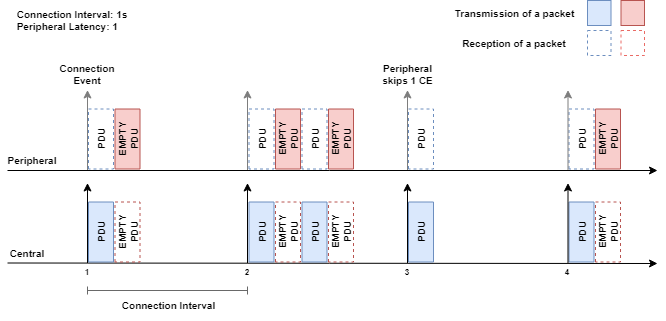
\includegraphics[width=0.8\textwidth,height=6cm,keepaspectratio=true]{images/conn_params/conn_params.drawio.png}
    \caption{
        Example of a timeline between a central and peripheral with CI=1s and PL=1. The CE at 1 second shows a normal connection event with one packet from the central and one response from the peripheral. The CE at 2 seconds shows how multiple transmissions can be changed during a single event. Finally, the CE at 3 seconds shows the peripheral using its PL of 1 to sleep during an event.
    }
    \label{fig:ci_and_pl}
\end{figure}

The most important parameters for the connection timing are \textit{connection interval} (CI), \textit{peripheral latency} (PL), and \textit{Supervision Timeout} (ST). The connection interval defines the time between periodic \textit{connection events} (CE). A connection event starts with a packet transmission from the central. Every packet from the central has to be followed by a packet from the peripheral. Multiple transmissions can be chained together in a single connection event. The peripheral latency defines how many connection events can be skipped by the peripheral to conserve energy. If a valid packet has not been received for more time than the supervision timeout defines, then a connection is considered broken. For example, take a CI of 1 second and a PL of 0. In that case, the central transmits a packet every second, and the peripheral responds. Now take a CI of 1 and a PL of 1. In this case, the central transmits every second, but the peripheral is allowed to sleep every other packet, effectively making the time between transmissions two seconds. The second example is displayed in Figure \ref{fig:ci_and_pl}. The units and ranges for the three connection parameters are defined in Table \ref{tbl:conn_params}.

\begin{table}
    \begin{center}
    \begin{tabular}{|l|l|l|l|}
        \hline
         & \textbf{Range} & \textbf{Unit} & \textbf{Real Range} \\
        \hline
        CI          & 0x0006 to 0x0C80 (hexadecimal) & 1.25ms &  7.5ms to 4000ms  \\
                    & 6 to 3200 (integer) & & \\
        \hline
        PL          & 0x0000 to 0x01F3 (hexadecimal) & N/A & N/A \\
                    & 0 to 499 (integer) & & \\
        \hline
        ST          & 0x000A to 0x0C80 (hexadecimal) & 10.00ms & 100ms to 32000ms \\
                    & 10 to 3200 (integer) & & \\
        \hline
    \end{tabular}
    \end{center}
    \caption{The three connection parameters which define the timing of connection events \cite{bluetooth_spec}. CI is the time in between connection events. PL defines how many connection events can be skipped by the peripheral. ST is the maximum time allowed since the last packet after which a connection is considered lost}
    \label{tbl:conn_params}
\end{table}


\subsubsection{Feature Expansion and Compliance}
Newer revisions of BLE can add new features to the link layer, adding new functionality or improving throughput. A vendor can also choose not to implement functionality not required for their application to reduce complexity. The supported features are stored in a 64-bit bitmask. The bitmask needs to be exchanged at the beginning of the connection to make sure a controller on one side does not use a procedure that the other controller does not support. Some examples of these features include \textit{LE Encryption} (bit 0), \textit{LE Data Packet Length Extension} (bit 5), \textit{LE 2MB PHY} (bit 11), and \textit{LE Coded PHY} (bit 11), which might sound familiar\cite[p. 2827]{bluetooth_spec}.

A feature that has been mentioned in the list above but not yet addressed is \textit{LE Data Packet Length Extension}. By default, the link layer packet data unit (PDU) allows for 27 bytes of data to be transmitted. The LE Data Packet Length Extension feature allows this to be increased up to 251 bytes for vastly improved throughput. However, higher-level protocols like ATT are encapsulated within the LL PDU, so the effective application data per packet will be lower than 251 bytes.

\subsection{Host Controller Interface}
The host controller interface provides a standardized way of communicating between the hardware-specific, real-time part of the stack (controller) and the rest, which is more hardware agnostic (host). The HCI can be implemented as a software API if the host and controller exist within the same silicon or using a hardware interface (UART, SPI, $\text{I}^{2}\text{C}$, USB) when the controller is a separate chip. It is common that the host and controller are implemented on the same chip since that reduces power consumption, which is often a large consideration for BLE devices.

The BLE specification defines a set of standardized HCI commands and events that the host and controller exchange with each other, together with a data packet format and control flow rules\cite{townsend_cufi}. Some vendors choose to extend the functionality of HCI by adding custom commands \cite{ti_ble_dev_guide}, which can allow the developer to control low-level settings of the radio.

\subsection{Logical Link Control and Adaption Protocol}
The task of the Logical Link Control and Adaption Protocol (L2CAP) layer is twofold. First, it encapsulates upper-level protocol packets into the standard LL PDUs, functioning as a multiplexer. The converse of this process is called decapsulation. The second function of L2CAP is fragmentation, which happens when an upper-level protocol packet exceeds the supported LL PDU size and has to be split into multiple L2CAP fragments. The L2CAP layer of the receiving side then has to defragment the packets to create the original packet. L2CAP adds a four byte header to each packet it encapsulates, thus reducing the effective packet data size further from 27 to 23 bytes.

\subsection{Security Manager}
The Security Manager (SM) layer contains both a protocol and a group of security-related algorithms and procedures. The algorithms are used to generate security keys that can be distributed using the defined procedures. Afterward, the Security Manager Protocol (SMP) can be used by other layers to safely connect and exchange data.

The following procedures are supported by the Security Manager:
\begin{itemize}
    \item \textit{Pairing} is when a set of temporary security keys are generated to encrypt the link.
    \item \textit{Bonding} can be done after \textit{pairing} by exchanging permanent security keys, which are stored in non-volatile memory.
    \item \textit{Encryption Re-establishment} is done to re-use previously stored permanent keys for a new encrypted link without having to \textit{pair} and \textit{bond}.
\end{itemize}

The pairing process requires the user to confirm the connection by entering a pin code from the peripheral on the central.

\subsection{Generic Access Profile}
The Generic Access Profile (GAP) layer defines the generic procedures related to the discovery of BLE devices and link management aspects of connecting to BLE devices. In addition, it also defines procedures required to attain certain security levels, as well as standard format requirements for parameters that are available at the user level. Most importantly, GAP defines certain \textit{roles} which govern the hierarchy of a BLE network, resulting in the asymmetric power requirements that allow the peripheral devices to operate efficiently.

\subsubsection{Roles}
GAP defines two pairs of roles for a total of four GAP roles. These pairs are the \textit{broadcaster} and \textit{observer} pair, and the \textit{peripheral} and \textit{central} pair.

A broadcaster is a device with a link layer set to advertising that only transmits data through advertisements of the \textit{non-connectable}. A device in the \textit{broadcasting role} should have a transmitter, but a receiver is optional. Devices that are suitable for broadcasting include temperature sensors and locating beacons.

An observer is a device that has its link layer state set to scanning and is only interested in reading advertisement packets without pursuing a connection. An observer should have a transmitter, but a receiver is optional. Phones are often observers when listening for BLE locating beacons to improve localization accuracy. 

A peripheral (GAP role) is any device that accepts connection requests from other devices. This means any device which is an advertiser sending out advertisements of the connectable type. When a peripheral (GAP role) goes to the connected link layer state, it changes from an advertiser (LL role) to a peripheral (LL role). A device in the \textit{peripheral role} should have a transmitter and a receiver.

A central (GAP role) is any device that initiates a connection with a peripheral. When central (GAP role) goes to the connected link layer state, it changes from an initiator (LL role) to a central (LL role). A device om the \textit{central role} should have a transmitter and a receiver.

Depending on the application requirements, a device may support multiple roles simultaneously. For example, a phone can be connected with wireless headphones, making it a central, and listening for locating beacons, making it an observer.

\subsection{Attribute Protocol and Generic Attribute Profile}
The Attribute Protocol (ATT) layer allows information to be discovered and transferred between BLE devices in a structured manner. ATT uses a client/server model, where the data is stored in the ATT server as attribute, and the client requests to read or manipulate the attribute data. Each attribute contains a known UUID used to identify the type of data contained in the attribute, and a 16-bit handle to identify the attribute itself. 

\begin{figure}[]
    \centering
    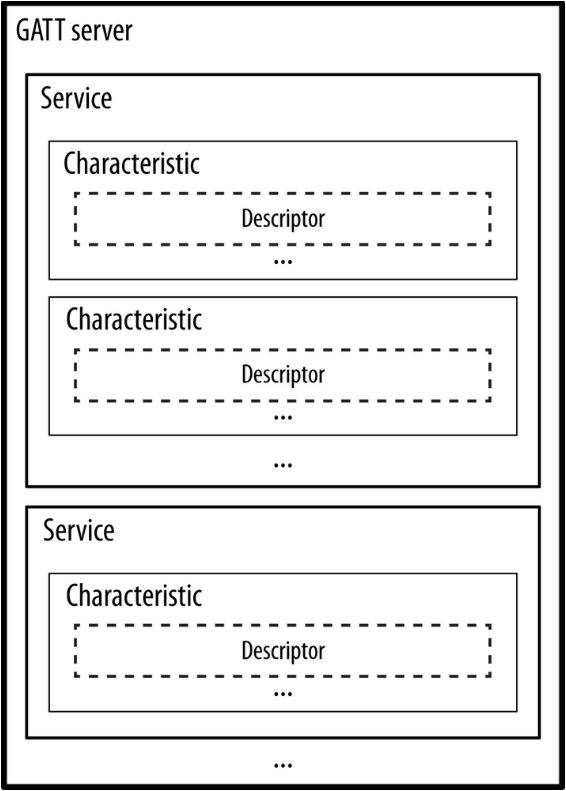
\includegraphics[width=0.5\textwidth,height=6cm,keepaspectratio=true]{images/gatt_service}
    \caption{
        The architecture of the GATT Server. Functionality is grouped as services. Services contain data as characteristics that can be read from or written to. Descriptors are used as metadata to describe characteristics and for configuring the server to notify the client of updates from the characteristic they are grouped under (Figure taken from \cite{townsend_cufi}).
    }
    \label{fig:gatt_server}
\end{figure}

The \textit{Generic Attribute Profile} extends the functionality of ATT by creating a hierarchy and data abstraction model on top of it. The GATT server groups attributes into \textit{Services}. Services contain data points called \textit{Characteristics}. These characteristics can be interpreted and configured using fields called \textit{Descriptors}. See Figure \ref{fig:gatt_server} for a schematic layout of the GATT Server. 

\begin{figure}[]
    \centering
    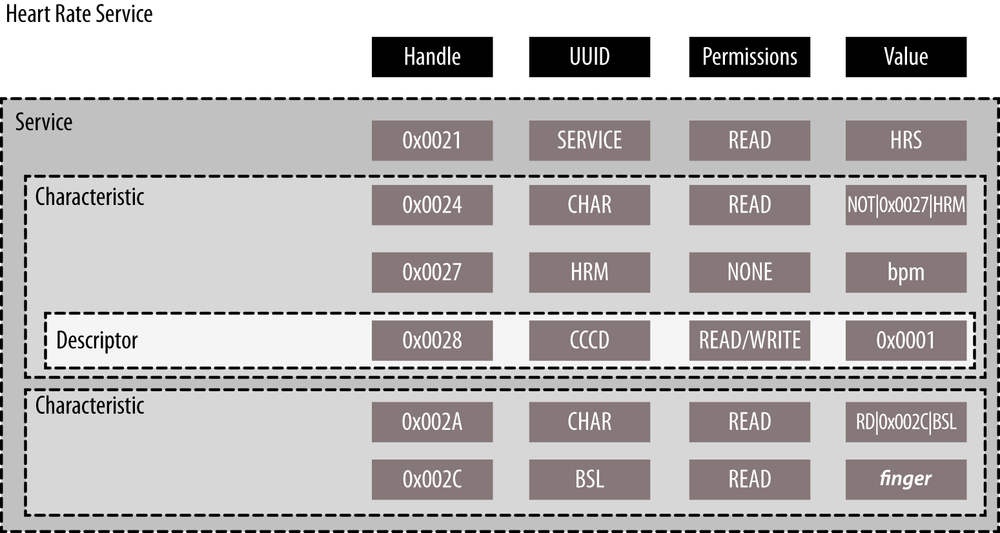
\includegraphics[width=0.5\textwidth,height=6cm,keepaspectratio=true]{images/heartrate_service}
    \caption{
        An example of a service. Each element is searchable through its UUID and then uniquely identifiable using its consecutively numbered handle \cite{townsend_cufi}.
    }
    \label{fig:hrs_layout}
\end{figure}
For a real-world example, see the Heart Rate Service (HRS) in Figure \ref{fig:hrs_layout}. The HRS allows a Client to read the heart rate sensor of a device. The HRS contains a characteristic called Heartrate. One of the descriptors tells us that the unit is defined as \textbf{beats per minute}. We could read the characteristic value manually, but if we would like to be notified when a new measurement is done, then we can set the Notify bit of the \textit{Client Characteristic Configuration} or CCC descriptor.

To be able to read or write to a characteristic, we need its handle. A handle is a number that is unique for a characteristic within a GATT Server. To find this handle, we can perform a \textit{Find By Type Request} using its 16-bit Universally Unique Identifier (UUID). Bluetooth SIG has predefined UUIDs for many predefined Services. Each predefined service has a specification that defines the shape of the service. This includes all the characteristics, descriptors, and their respective UUIDs.

The process of finding all these handles is what is called \textit{Service Discovery}. The result of this process is a list of handles that can be used to read and write to the server. After Service Discovery is done, the GATT Servers need to be configured. This usually means writing to the CCC descriptor to configure notifications for the desired characteristics. This process will, from here on, be referred to as Configuration. 

Both the Central and the Peripheral can be Servers and Clients at the same time. For example, a phone can provide the central time for a smartwatch to display on the watch face, while the smartwatch measures the heart rate for the phone to present within a health application. This means that a Service Discovery and Configuration need to be performed by both the Central and the Peripheral.

\section{Operating Systems Used to Implement the System Proposed}
The FreeBie project was originally developed using the open-source BLE stack Packetcraft \cite{packetcraft}. Packetcraft is a \textit{real-time operating system} (RTOS), which means it allows for real-time scheduling of tasks. Real-time scheduling is essential to run the link layer controller. Due to its architecture, it was especially suitable to be modified in the way required for intermittent operation. This is because all OS tasks are managed using a single scheduler which uses a generic sleep method. This sleep method was altered to configure the real-time clock (RTC), save the memory to FRAM, and fully power down the System-on-Chip (SoC).

However, since FreeBie was originally developed, Packetcraft has gone into closed-source development. For this reason, a newer RTOS was chosen for the central, called Zephyr. Zephyr OS is a modern RTOS developed by the Linux Foundation and is now the officially supported stack for Nordic Semiconductors \cite{zephyrproject}. A side-effect of implementing the proposed solutions on two platforms is proving that the approach used to solve the issues outlined in Section \ref{sec:introduction_problem_statement} is platform-agnostic.

\section{Demo System}
\label{sec:demo_application}

\begin{figure}
    \centering
    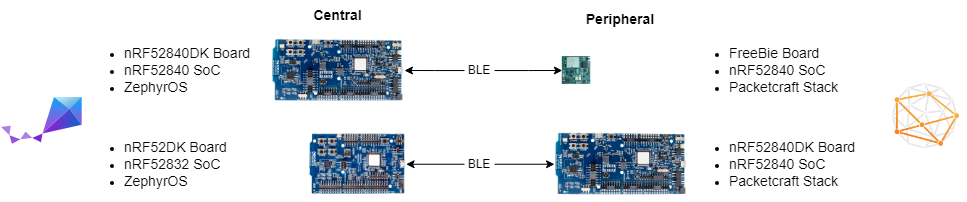
\includegraphics[width=1\textwidth,height=6cm,keepaspectratio=true]{images/demo_layout/demo_layout.drawio.png}
    \caption{
        The combination of central and peripheral on top is used for testing, while the combination on the bottom is used for development.
    }
    \label{fig:demo_layout}
\end{figure}
The modifications we aim to make to the system will attempt to remove certain procedures without losing their functionality. We have developed a demo system to verify that these functions still work. The demo system consists of a single central and peripheral, shown in Figure \ref{fig:demo_layout}. The configuration on top consisted of an nRF52840DK as a central and the FreeBie as a peripheral and was mostly used when verifying new code, when intermittency was required, or during the final testing phase and evaluation. The configuration on the bottom was primarily used during development since the FreeBie codebase runs on any nRF52840DK when intermittent operation is disabled. This configuration allows us to access the serial debug trace of Packetcraft. 

We developed a Packetcraft application for FreeBie to act like a smartwatch peripheral and a Zephyr application for the central to work like a stand-in for a phone. Appendix \ref{app:appendix_a} contains a list of all available terminal commands, a list of all available services and characteristics, as well as a description of how to use the demo system and how it was developed. 